In this chapter the process of loading individual levels will be explained.
This involves loading the level, encoded as an image in the PNG format, parsing values from this format, and finally placing tiles in the game world representing those values.

\section{Designing and loading levels}
Level creation is an important aspect when developing a game, and for this project there are different elements to consider for the level creation workflow.
\begin{itemize}
    \item The development process is agile, meaning the level should be easily modifiable to adapt to changes
    \item Game balancing, requiring the production of levels at a sufficient pace in order to quickly iterate on game balancing topics, such as strategies for a particular map layout
    \item The project has no dedicated level designer whom we can allocate to finely tune and manually design levels
\end{itemize}
These elements sets up some different challenges to the project.
To keep up with potential changes, a quick way to create levels is preferred for the following reasons:
\begin{itemize}
    \item Designing levels and placing gameobjects in the Editor does not afford quick iterations, as required by our development process
    \item The Editor does not afford easy refactoring of large levels, in that objects must be moved or replaced manually. \textit{Large} is relative, but for our purposes it could be upwards +10.000 gameobjects
    \item Individual levels would have to reside in individual \texttt{Scene} files, increasing the complexity of collaboration since scenefiles does not  automatically merge correct in version control systems.
\end{itemize}

While there are different approaches for circumventing the above inconveniences, our solution is to encode the layout of each individual level in an external file which is then loaded and interpreted.
Historically, game developers have often used this approach, usually encoded in some in-house binary format~\cite{quake-bsp-format}.
While customized in-house format would offer significant flexibility, but it would also result in additional development, if the players should have the option to create their own levels, as a custom level editor would be necessary.
Instead the choice of encoding the map in the PNG format was made, as described in section \ref{sec:modules:missions:customcontent}.
Using the PNG format, it is only a matter of specifying \textit{what} a particular color should encode and interpreting that color when loading a level.
As an example, the following could specify how colors could be specified to encode information about a level:
\begin{itemize}
    \item Black would be ground
    \item Green is grass
    \item Red is building floor
    \item And yellow being building walls.
\end{itemize}
One obvious shortcoming from the above example is the lack of variation - maybe one would like to be able to specify different types of walls or floors. This could however be mitigated by either specifying more colors or by interpreting a color differently depending on the context of the pixel.
To introduce variety into our levels, we use the latter approach for some colors, which we will describe later in this chapter.
\\

Having decided on the format and encoded color values, we can design levels such as seen in figure~\ref{fig:png_map}.

\begin{figure}[H]
    \centering
    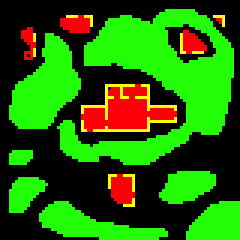
\includegraphics[width=1\textwidth]{figures/generating_levels/map.png}
    \caption{A PNG image encoding a level}
    \label{fig:png_map}
\end{figure}
By looking at Figure~\ref{fig:png_map}, it is illustrated that there are some patches of grass, a building in the middle of the map and some torn-down buildings in the periphery of the map encoded in the PNG.
A single blue pixels encodes where the crafting table should be placed within the level.
\\\\
The color values can then be interpreted into distinct integer values in a two-dimensional array, as seen in Figure~\ref{fig:png_to_array}.
%thread carefully below...
\begin{figure}[H]
    \centering
    \begin{tabular}{cc}
        {\footnotesize
            \setlength{\tabcolsep}{4.5pt}
            \begin{tabular}{|c|c|c|c|c|c|c|c|c|c|}
                \hline
                \cellcolor{black} & \cellcolor{black} & \cellcolor{black} &
                \cellcolor{black} & \cellcolor{black} & \cellcolor{red} &
                \cellcolor{red} & \cellcolor{red} & \cellcolor{red} &
                \cellcolor{red} \\ \hline
                \cellcolor{green} & \cellcolor{green} & \cellcolor{black} &
                \cellcolor{black} & \cellcolor{black} & \cellcolor{yellow} &
                \cellcolor{red} & \cellcolor{red} & \cellcolor{red} &
                \cellcolor{red} \\ \hline
                \cellcolor{green} & \cellcolor{green} & \cellcolor{green} &
                \cellcolor{black} & \cellcolor{black} & \cellcolor{yellow} &
                \cellcolor{red} & \cellcolor{red} & \cellcolor{red} &
                \cellcolor{red} \\ \hline
                \cellcolor{green} & \cellcolor{green} & \cellcolor{green} &
                \cellcolor{black} & \cellcolor{black} & \cellcolor{yellow} &
                \cellcolor{red} & \cellcolor{red} & \cellcolor{red} &
                \cellcolor{red} \\ \hline
                \cellcolor{green} & \cellcolor{green} & \cellcolor{green} &
                \cellcolor{black} & \cellcolor{black} & \cellcolor{yellow} &
                \cellcolor{yellow} & \cellcolor{red} & \cellcolor{red} &
                \cellcolor{yellow} \\ \hline
                \cellcolor{green} & \cellcolor{green} & \cellcolor{green} &
                \cellcolor{black} & \cellcolor{black} & \cellcolor{black} &
                \cellcolor{black} & \cellcolor{black} & \cellcolor{black} &
                \cellcolor{black} \\ \hline
                \cellcolor{green} & \cellcolor{green} & \cellcolor{green} &
                \cellcolor{green} & \cellcolor{black} & \cellcolor{black} &
                \cellcolor{black} & \cellcolor{black} & \cellcolor{black} &
                \cellcolor{black} \\ \hline
                \cellcolor{green} & \cellcolor{green} & \cellcolor{green} &
                \cellcolor{green} & \cellcolor{black} & \cellcolor{black} &
                \cellcolor{black} & \cellcolor{black} & \cellcolor{black} &
                \cellcolor{black} \\ \hline
                \cellcolor{green} & \cellcolor{green} & \cellcolor{green} &
                \cellcolor{green} & \cellcolor{green} & \cellcolor{black} &
                \cellcolor{black} & \cellcolor{black} & \cellcolor{black} &
                \cellcolor{black} \\ \hline
                \cellcolor{green} & \cellcolor{green} & \cellcolor{green} &
                \cellcolor{green} & \cellcolor{green} & \cellcolor{green} &
                \cellcolor{green} & \cellcolor{green} & \cellcolor{green} &
                \cellcolor{black} \\ \hline
            \end{tabular}
        }
        &
        {\footnotesize
            \setlength{\tabcolsep}{2.5pt}
            \begin{tabular}{|c|c|c|c|c|c|c|c|c|c|}
                \hline
                0 & 0 & 0 & 0 & 0 & 4 & 4 & 4 & 4 & 4 \\ \hline
                1 & 1 & 0 & 0 & 0 & 3 & 4 & 4 & 4 & 4 \\ \hline
                1 & 1 & 1 & 0 & 0 & 3 & 4 & 4 & 4 & 4 \\ \hline
                1 & 1 & 1 & 0 & 0 & 3 & 4 & 4 & 4 & 4 \\ \hline
                1 & 1 & 1 & 0 & 0 & 3 & 3 & 4 & 4 & 3 \\ \hline
                1 & 1 & 1 & 0 & 0 & 0 & 0 & 0 & 0 & 0 \\ \hline
                1 & 1 & 1 & 1 & 0 & 0 & 0 & 0 & 0 & 0 \\ \hline
                1 & 1 & 1 & 1 & 0 & 0 & 0 & 0 & 0 & 0 \\ \hline
                1 & 1 & 1 & 1 & 1 & 0 & 0 & 0 & 0 & 0 \\ \hline
                1 & 1 & 1 & 1 & 1 & 1 & 1 & 1 & 1 & 0 \\ \hline
            \end{tabular}
        }
    \end{tabular}
    \caption{Interpreting a PNG map image into a two-dimensional array}\label{fig:png_to_array} 
\end{figure}
Values are then further separated into a new two-dimensional array consisting of only each individual value, as illustrated on the right side in Figure \ref{fig:png_to_array}.
The data within those arrays are what we use to generate tiles and some game entities within the gameworld.

\section{Generating level backdrop}
As explained previously, our game is a top-down 2D action game.
Important to note is the top-down 2D aspect of it when we are to generate our levels.
A historical, and still prevalent technique for 2D games, is using a tiling approach for the layout of both the backdrop of the level and entities within it.
Several different approaches to tiling have been used in games, including squares, isometric and hexagonal tiles.
Figures~\ref{fig:civ-1_square},~\ref{fig:civ-2_iso}~and~\ref{fig:wesnoth_hex}
show examples of games using each of the mentioned techniques of tiling.

\begin{figure}[H]
    \centering
    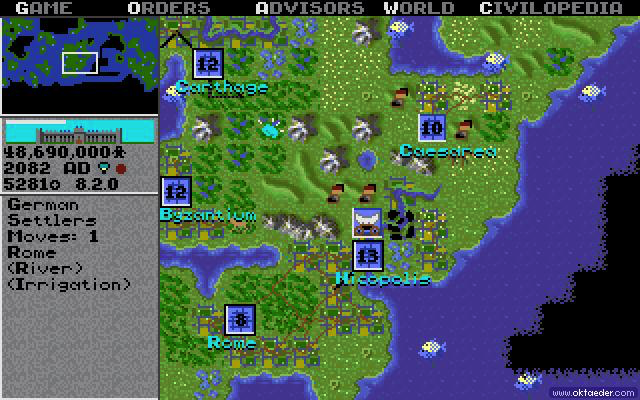
\includegraphics[width=0.5\textwidth]{figures/generating_levels/civ-1_square.png}
    \caption{Civilizations 1, using squares as tiles}\label{fig:civ-1_square}
\end{figure}

\begin{figure}[H]
    \centering
    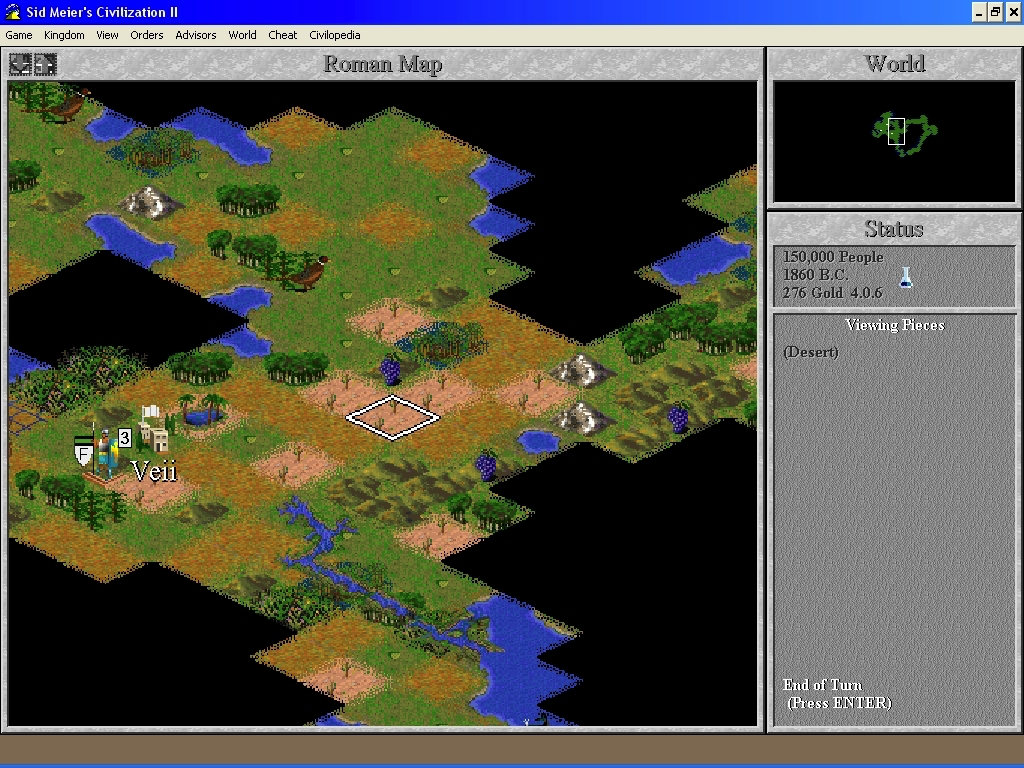
\includegraphics[width=0.5\textwidth]{figures/generating_levels/civ-2_iso.png}
    \caption{Civilizations 2, using the isometric technique}\label{fig:civ-2_iso}
\end{figure}

\begin{figure}[H]
    \centering
    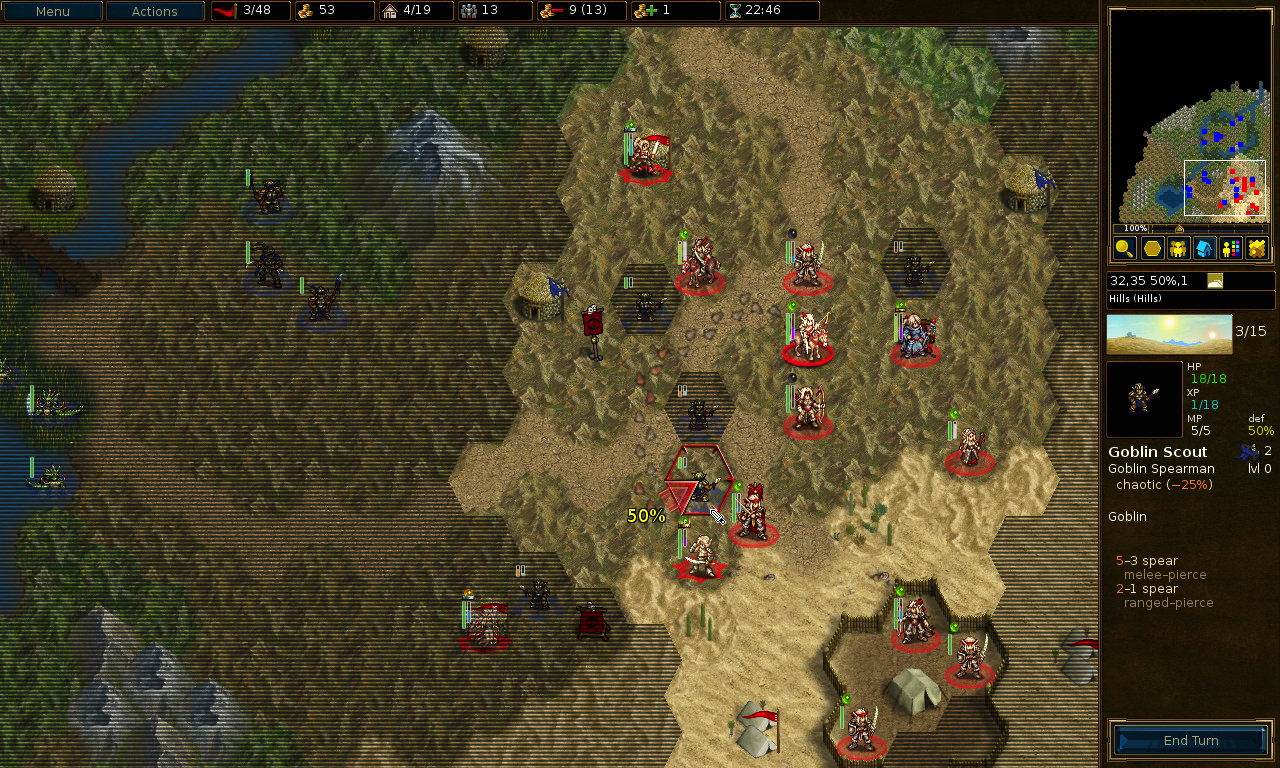
\includegraphics[width=0.5\textwidth]{figures/generating_levels/wesnoth_hex.png}
    \caption{Battle of Wesnoth, using a hexagonal tiling technique}\label{fig:wesnoth_hex}
\end{figure}
Since the individual techniques mostly impact the visual appearance of the game, the underlying data structures remain the same.
We have chosen to apply the most straightforward tiling technique: square tiles.
\\
\\
The first naive implementation that we prototyped, was to iterate through the two-dimensional map and place tiles corresponding to the values, with tiles being \texttt{sprites} in the gameworld.
In Unity sprites needs to be assigned a \texttt{sprite renderer} component which in turn needs to be attached a \texttt{gameobject}.
This effectively means that for each tile, an instantiation a gameobject has to be made, which easily can get expensive in computation.

Since tiles exhibit no particular behavior, it seems excessive to instantiate gameobjects for each tile.
Not only that, but we were experiencing performance implications on mobile devices using this method.
It is possible to substantially reduce the gameobjects required to be instantiated by \textit{grouping} similar areas into bigger tiles.
To do this, the map needs to be grouped such that large area consisting of only one type will be marked with a similar value in the data structure.
The groups are then \textit{blitted} together in a tile-pattern to form a larger texture.
There is a technical limit to this technique however, as texture-resolutions are limited by hardware. For our implementation, we limit the resolution of larger textures to $1024 x 1024$, as that would be within the bounds of the capabilities of the target hardware.
A comparison of the result of the two techniques can be seen in figure~\ref{fig:grouped_tiling_comparison}.
\begin{figure}[H]
    \centering
    \begin{tabular}{cc}
        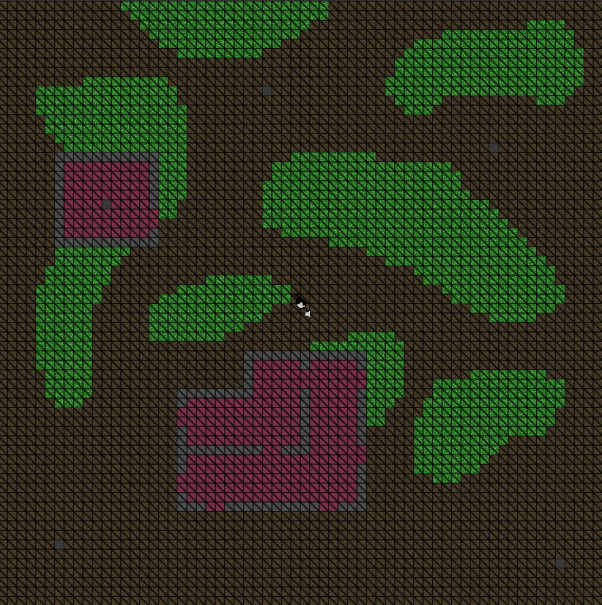
\includegraphics[width=0.5\textwidth]{figures/generating_levels/naive-tile.png}
        &
        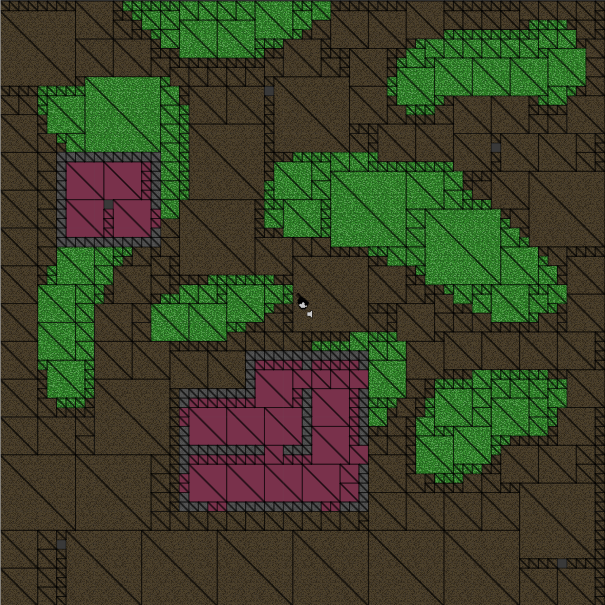
\includegraphics[width=0.5\textwidth]{figures/generating_levels/grouped-tile.png}
    \end{tabular}
    \caption{(left) naive tiling, (right) grouping tiles into larger tiles}\label{fig:grouped_tiling_comparison}
\end{figure}
The computation involved in blitting textures together \textit{can} be significant on mobile devices, as the larger textures have to be uploaded to the GPU in order to reflect changes.
The blitting is performed during runtime whenever a map is loaded, so in order to avoid blitting the same texture more than once, a caching of the larger textures to disk is performed, such that they can be loaded between subsequent runs of the application.
By caching and loading already blitted textures to disk, we significantly reduced loading times on mobile devices.
\todomichael{What were the improviements? Do we have any numbers? logs?}
\todobrian{We did see improvements in shorter loading times. I can do measurements of this if you want to haz?}
\\
\\
\textit{Transition} tiles between certain type of tiles, in particular between grass and ground, are desired.
This technique is also used in the games seen in figures~\ref{fig:civ-1_square},~\ref{fig:civ-2_iso}~and~\ref{fig:wesnoth_hex}.
To achieve this, an adaptation of the \textit{Marching squares} algorithm is used, and marks a position in the data structure as a particular type, based on the values of its neighbouring values~\cite{marching-squares}.
A corresponding \textit{transition tile} is then blitted together, cached to disk in the same manner as grouped tiles, and assigned to the gameobject at that position.
Figure~\ref{fig:transition_comparison} shows a comparison before and after integrating the algorithm.
\todobrian{reconsider ref for marching squares}

\begin{figure}[H]
    \centering
    \begin{tabular}{cc}
        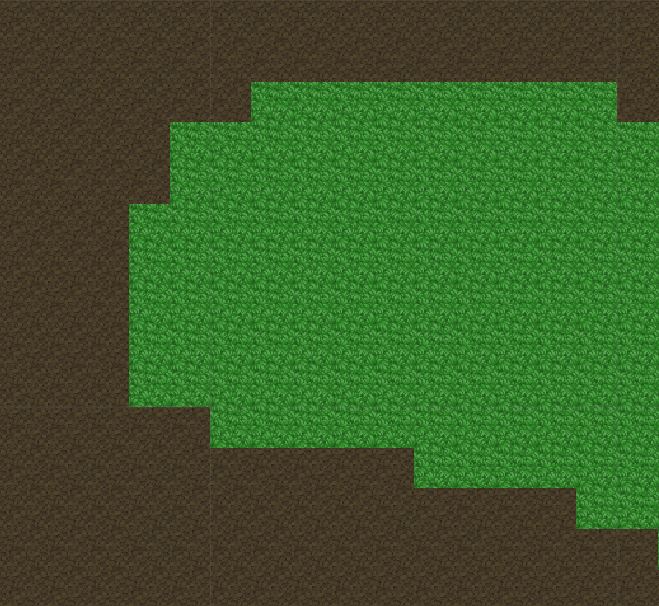
\includegraphics[width=0.5\textwidth]{figures/generating_levels/no_transition.png}
        &
        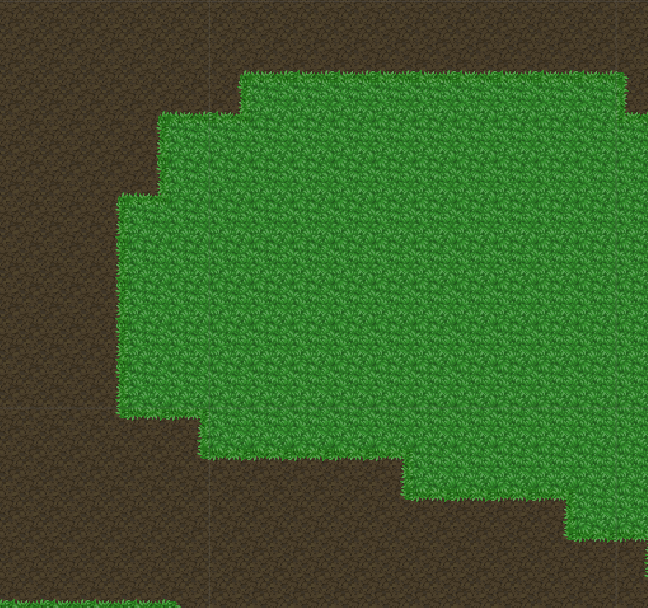
\includegraphics[width=0.5\textwidth]{figures/generating_levels/with_transition.png}
    \end{tabular}
    \caption{(left) without transitioning, (right) with transitioning tiles}\label{fig:transition_comparison}
\end{figure}

\section{Placing walls and colliders}
Placing walls involves both placing them as textured tiles within the gameworld, and placing \textit{colliders} such that moving object in the game cannot move through them.

\subsection{Placing wall sprites}
A naive implementation for placing wall-sprites within the gameworld is to place a gameobject with the texture of a wall.
However, the walls should fit seamlessly together as a homogeneous unit.
This is done using an adaptation of the \textit{Marching squares}, following the same procedure as with transitional tiles between grass and ground.
Firstly it is detected if a wall is a ``stump'', a regular vertical or horizontal middle section or a t-section. 
Diagonal walls are treated as ''stumps'', so our marching squares adaptation only considers adjacent tiles at 90-degree angles.
Figure~\ref{fig:wall_comparison} illustrates an example of placing walls where tiles are not ``connected'' and one where tiles are ``connected'' and figure~\ref{fig:walls_ingame} showing an in-game example.

\begin{figure}[H]
    \centering
    \begin{tabular}{cc}
        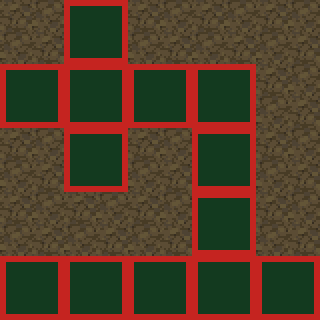
\includegraphics[width=0.5\textwidth]{figures/generating_levels/wall_no_border.png}
        &
        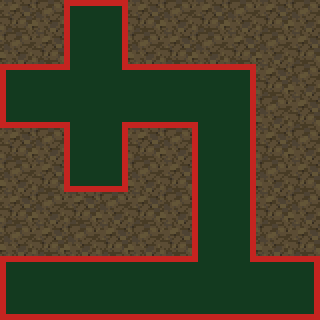
\includegraphics[width=0.5\textwidth]{figures/generating_levels/wall_with_border.png}
    \end{tabular}
    \caption{(left) not connected, and (right) where walls are connected}\label{fig:wall_comparison}
\end{figure}

\begin{figure}[H]
    \centering
    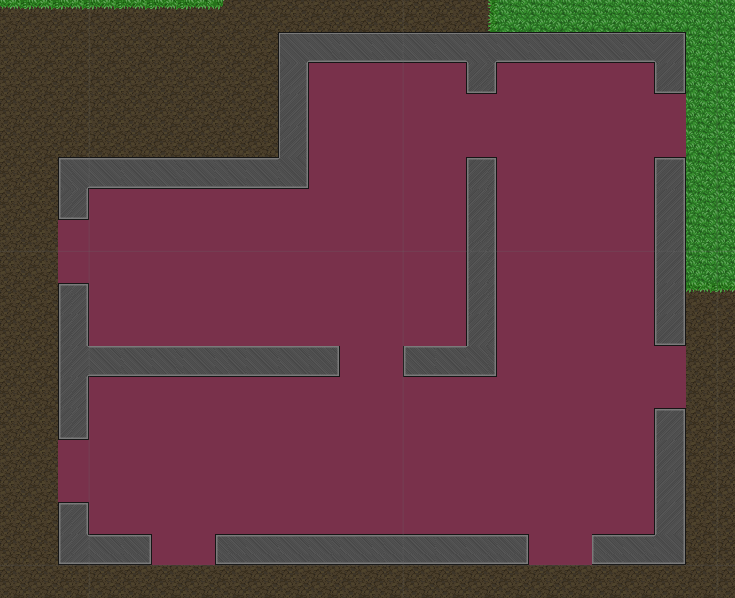
\includegraphics[width=0.5\textwidth]{figures/generating_levels/walls_ingame.png}
    \caption{In-game example of connected walls}\label{fig:walls_ingame} 
\end{figure}

\subsection{Placing wall colliders}
For wall colliders it is desired to find the contour of walls into gameobjects assigned a collide-able component in the gameworld.
The first naive implementation is to place a square collider (regular \texttt{Collider2D}) for each wall tile.
An example of placing colliders at each wall tile can be seen in figure~\ref{fig:wall_with_vertices}.
This resulted in the unfortunate behaviour that collisions from rigidbodies - the player and enemies - behaved unreliable and rigid bodies would ``bounce off'' the walls whenever they would be ``between'' two collider sections.
\\
A solution to this problem is to place \texttt{Polygon Collider2D}s, using the contour vertices of the colliders shown in figure~\ref{fig:wall_with_vertices}. 
However this reveals another problem: the resulting polygon is concave.
This means that the polygon cannot \textit{easily} be constructed only knowing the vertices.
Our solution was to use an adaptation of \textit{flood fill} to first find connected vertical and then horizontal wall sections.
From the algorithm, we can find contour vertices for convex polygons which are \textit{larger} than single wall sections.
This significantly reduces the number of colliders necessary and eliminating the mentioned problem of unreliable behavior for rigidbodies colliding with walls.
An \textit{optimal} solution would be to construct a concave polygon from the vertices, which would require finding all
contour vertices \textit{and} the order in which they should connected when constructing the polygon.
The result of our \textit{flood fill} approach can be seen in figure~\ref{fig:wall_with_convex}.

\begin{figure}[H]
    \centering
    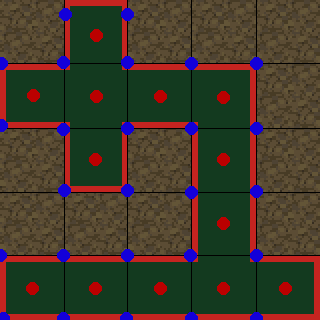
\includegraphics[width=0.5\textwidth]{figures/generating_levels/wall_with_vertices.png}
    \caption{Placing colliders at tile positions}\label{fig:wall_with_vertices} 
\end{figure}

\begin{figure}[H]
    \centering
    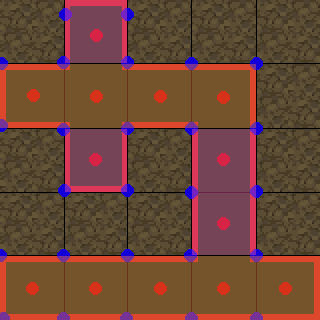
\includegraphics[width=0.5\textwidth]{figures/generating_levels/wall_with_convex.png}
    \caption{Finding connected concave polygons using flood fill}\label{fig:wall_with_convex} 
\end{figure}
